% =====================================================================
%  Figures for "Conformance-Aware HTN Domain Repair"
%  \input this file; figures live in figures/out/*.pdf (vector) and *.png.
%  Each block: a comment noting the driving result file + the claim it
%  supports, then the figure environment with a one-sentence caption.
%  Requires \usepackage{graphicx}.  Suggested: \graphicspath{{figures/out/}}
%  No chart has a title/subtitle (the takeaway lives in the caption).
% =====================================================================

% ---------------------------------------------------------------------
% FIGURE 1 / OVERVIEW (schematic).  Driven by: results/po_indifference.json for
% the annotated precision values (cost_only_worst..cost_only_expected = 0.23..0.55,
% conformance = 1.0); the flow itself is conceptual.  Supports the paper thesis:
% a flawed domain + target admits many minimal-cost repairs that all re-derive the
% target, the cost-only objective is indifferent among them (C1 / Prop 1), and the
% conformance-aware repair restores exactly the gold behaviour (C3).
% ---------------------------------------------------------------------
\begin{figure}[t]
  \centering
  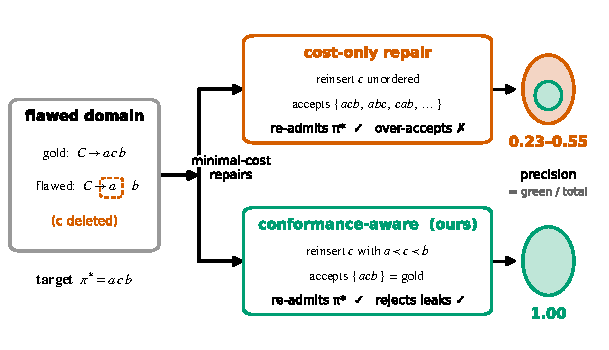
\includegraphics[width=\columnwidth]{figures/out/fig_overview.pdf}
  \caption{Repairing a flawed HTN domain so the target plan $\pi^{*}$ is again
  derivable admits many equal-cost repairs; the cost-only objective is indifferent
  among them and may pick one that over-accepts invalid orderings (measured
  precision $0.23$--$0.55$ across the IPC partial-order benchmark), whereas the
  conformance-aware repair re-admits $\pi^{*}$ while rejecting the leaks
  (precision $1.0$). The right-hand lens shows each repair's accepted language as
  area --- green is the gold behaviour, the vermillion halo is what is wrongly
  accepted --- so precision is the green fraction.}
  \label{fig:overview}
\end{figure}

% ---------------------------------------------------------------------
% MECHANISM.  Driven by: data/synthetic.py + CLAUDE.md (the _leak_gadget;
% gold language {a crit b, b crit a}).  Supports the claim that the gap has
% a single structural cause -- a shared compound -- and that the re-inserted
% action's PLACEMENT decides conformant vs leaky (Sec. "why the gap exists").
% ---------------------------------------------------------------------
\begin{figure}[t]
  \centering
  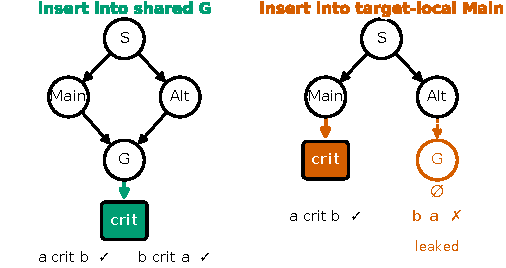
\includegraphics[width=\columnwidth]{figures/out/fig_leak_tree.pdf}
  \caption{The conformance gap has one structural cause: inserting the deleted
  action into the \emph{shared} compound $G$ recovers the gold language, while
  inserting it into the target-local method \textsf{Main} makes the target
  derivable yet lets the \textsf{Alt} branch leak the gold-rejected trace
  ``\textsf{b a}''.}
  \label{fig:leak}
\end{figure}

% ---------------------------------------------------------------------
% E1 CONFORMANCE GAP.  Driven by: results/headline.json
% (experiment_1_conformance_gap, regime=gold_structural).  Supports: the gap is
% present in every structurally-ambiguous family and exactly zero in the
% ambiguity-free control (the evaluator does not manufacture failures).
% ---------------------------------------------------------------------
\begin{figure}[t]
  \centering
  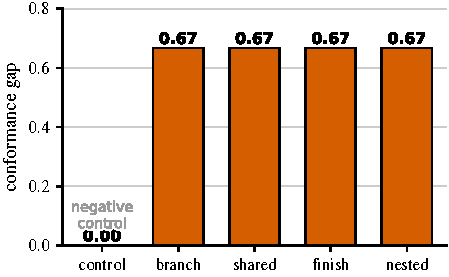
\includegraphics[width=\columnwidth]{figures/out/fig_conformance_gap.pdf}
  \caption{Two of every three minimum-cost target-valid repairs over-accept in
  each structurally-ambiguous family, and none do in the ambiguity-free
  control.}
  \label{fig:gap}
\end{figure}

% ---------------------------------------------------------------------
% INVISIBILITY (methodological).  Driven by: results/headline.json
% (gap by family x negative-generation regime).  Supports: the gap is invisible
% to target-local negatives and visible only under gold-structural negatives;
% the control stays at zero under all regimes.
% ---------------------------------------------------------------------
\begin{figure}[t]
  \centering
  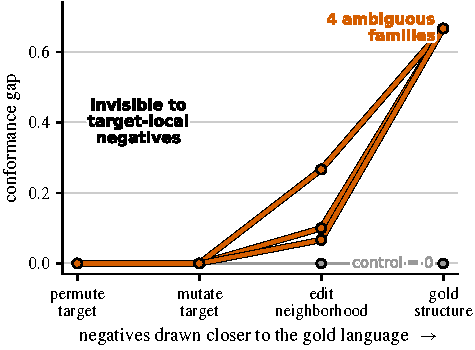
\includegraphics[width=\columnwidth]{figures/out/fig_invisibility.pdf}
  \caption{Whether the gap is seen at all depends on where negatives come from:
  it grows as negatives approach the gold language---permuting or mutating the
  target reports nothing and editing it only a fraction, while only
  gold-structural negatives expose the full gap and the control never leaves the
  floor.}
  \label{fig:invisible}
\end{figure}

% ---------------------------------------------------------------------
% E2 SELECTOR.  Driven by: results/selector_comparison.json (regime=
% gold_structural; cost-only expected/worst vs conformance, fitness=1.0).
% Supports: at equal recall, conformance selection reaches precision 1.0 where
% the cost-only objective's expected precision over its own indifference set
% falls short.
% ---------------------------------------------------------------------
\begin{figure}[t]
  \centering
  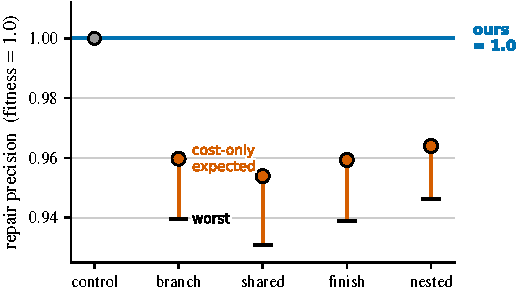
\includegraphics[width=\columnwidth]{figures/out/fig_precision_gain.pdf}
  \caption{At identical fitness, conformance-aware selection attains precision
  $1.0$ on every family, whereas the cost-only objective is indifferent across a
  min-cost set whose expected (and worst-case) precision is strictly lower.}
  \label{fig:gain}
\end{figure}

% ---------------------------------------------------------------------
% E4 TWO LAYERS.  Driven by: results/timeline_conformance.json +
% results/headline.json.  Supports: an independent Allen-timeline layer flags
% the same ambiguous families and leaves the control at zero (two orthogonal,
% both-controlled axes).
% ---------------------------------------------------------------------
\begin{figure}[t]
  \centering
  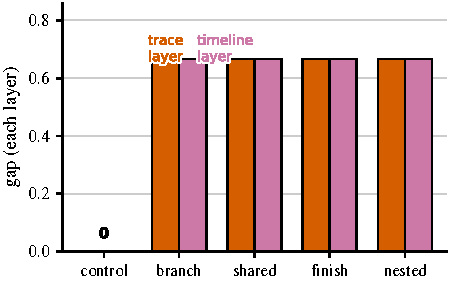
\includegraphics[width=\columnwidth]{figures/out/fig_timeline_gap.pdf}
  \caption{An independent temporal (Allen-interval) verification layer reports
  the same gap as the trace layer on every family, including a clean zero on the
  control.}
  \label{fig:timeline}
\end{figure}

% ---------------------------------------------------------------------
% REAL-IPC CENTERPIECE.  Driven by: results/ipc_overgen_openai-o4-mini-high.jsonl
% and results/ipc_overgen_openai-gpt-oss-120b-high.jsonl (length-matched
% escaping-edges precision; gold-pruned control = 1.0).  Supports: on real IPC,
% SOTA minimal-cost repairs admit a mostly-invalid length-L plan language.
% ---------------------------------------------------------------------
\begin{figure}[t]
  \centering
  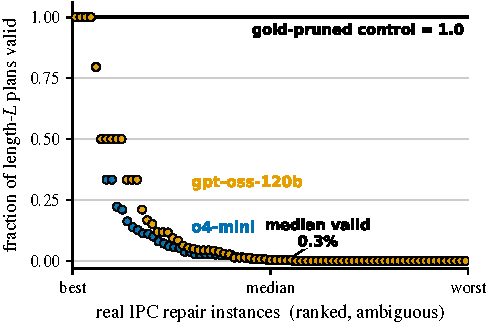
\includegraphics[width=\columnwidth]{figures/out/fig_overgen_cliff.pdf}
  \caption{On real IPC-2020 instances, the published o4-mini and gpt-oss-120b
  repairs admit a length-$L$ plan language that is a median $0.3\%$ valid---two
  independent models on the same floor, versus the gold-pruned control at
  $1.0$.}
  \label{fig:cliff}
\end{figure}

% ---------------------------------------------------------------------
% COST-PRECISION FRONTIER (theory).  Driven by: results/frontier.json
% (precision vs insertion cost as gold structure is restored, real IPC).
% Supports: cost and precision are in fundamental tension; minimal-cost repair
% sits at the precision floor and precision is bought only near full recovery.
% ---------------------------------------------------------------------
\begin{figure}[t]
  \centering
  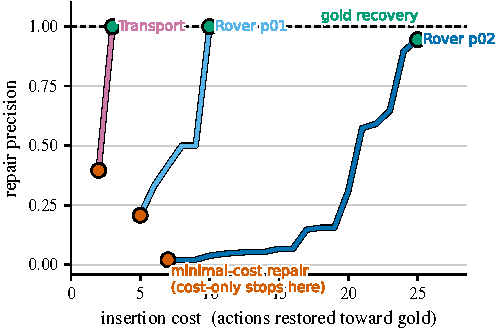
\includegraphics[width=\columnwidth]{figures/out/fig_frontier.pdf}
  \caption{Precision is bought only by restoring nearly all of the gold
  structure: the minimum-cost repair, where the cost-only objective stops, sits
  at the precision floor of the cost-precision frontier.}
  \label{fig:frontier}
\end{figure}

% ---------------------------------------------------------------------
% TO/PO CONTRAST (schematic).  No data.  Supports the Sec. 4 reversal remark:
% reordering over-acceptance is a partial-order phenomenon -- a TO reinsertion
% fixes order by position (no gap), a PO reinsertion may omit the cost-free
% precedence constraints (gap), which is also why CEGIS is PO-specific.
% ---------------------------------------------------------------------
\begin{figure}[t]
  \centering
  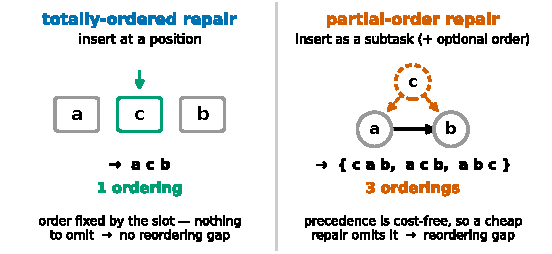
\includegraphics[width=\columnwidth]{figures/out/fig_to_vs_po.pdf}
  \caption{Reordering over-acceptance is specific to partial order: a
  totally-ordered repair inserts the action at a \emph{position}, fixing every
  action's order (one linearization), whereas a partial-order repair inserts it as a
  subtask whose precedence constraints are cost-free and may be omitted, leaving it
  unordered and admitting gold-rejected linearizations.}
  \label{fig:tovspo}
\end{figure}

% ---------------------------------------------------------------------
% CEGIS MECHANISM (schematic, real instance).  Driven by: a real Monroe-FO method
% (m_repair_line_with_tree); linearization counts + precisions are COMPUTED from its
% gold order via the same subset-DP counter as results/po_cegis.json.  Supports:
% Prop 2 / C3-PO' -- each counter-example pins exactly one missing precedence edge,
% so CEGIS recovers gold ordering in #missing-edges steps (optimal).
% ---------------------------------------------------------------------
\begin{figure}[t]
  \centering
  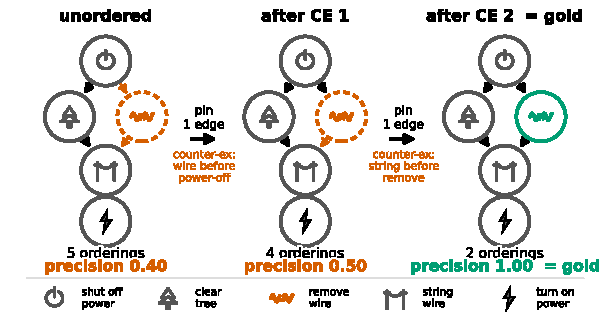
\includegraphics[width=\columnwidth]{figures/out/fig_cegis_loop.pdf}
  \caption{Counter-example-guided precedence recovery on a real partial-order method
  (Monroe \textsf{m\_repair\_line\_with\_tree}): the unordered reinsertion of
  \textsf{remove-wire} admits five orderings (precision $0.40$); each counter-example
  -- e.g.\ \emph{remove-wire before shut-off} -- pins exactly one missing precedence
  edge, and two such edges recover the gold order (precision $1.0$), which is optimal.}
  \label{fig:cegisloop}
\end{figure}

% ---------------------------------------------------------------------
% METHOD + TO/PO REVERSAL.  Driven by: results/po_indifference.json (fair
% cost-only baseline: expected + worst over the enumerated indifference set, per
% domain and for the genuinely-partial-order subset) and results/po_cegis.json
% (CEGIS precision + counter-examples).  Full 9-domain corpus, 334 methods / 775
% primitive-removal instances.  Supports: counter-example-guided conformance
% repair recovers gold ordering optimally on PO (~1.4 counter-examples = #missing
% precedence edges); the gap is LARGER on genuinely partial-order gold (Monroe);
% and there is no reordering gap to close on TO.
% ---------------------------------------------------------------------
\begin{figure}[t]
  \centering
  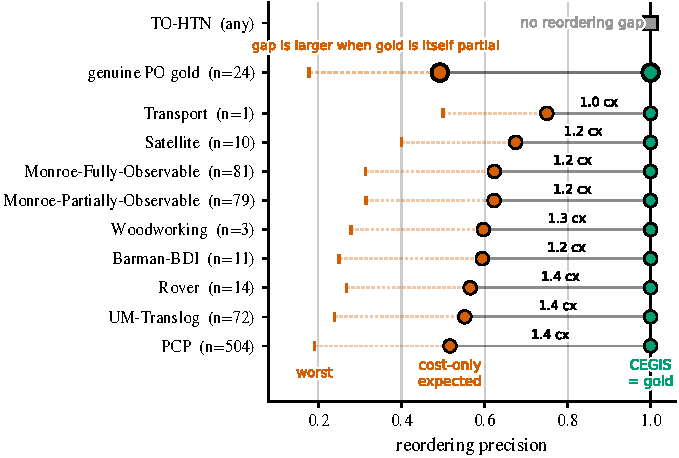
\includegraphics[width=\columnwidth]{figures/out/fig_cegis.pdf}
  \caption{On partial-order HTN, counter-example-guided conformance repair lifts
  reordering precision from the fair cost-only baseline (expected $0.55$, worst
  $0.23$ over $775$ primitive-removal instances) to $1.0$ with $\approx\!1.4$
  counter-examples (the number of missing precedence constraints, i.e.\ optimal);
  the gap is \emph{larger} on the genuinely partial-order methods where gold itself
  has reordering freedom (expected $0.49$), and on totally-ordered HTN there is no
  reordering gap to close.}
  \label{fig:cegis}
\end{figure}

% ---------------------------------------------------------------------
% COMPOUNDING.  Driven by: results/po_fulldomain_raw.json (per-derivation
% length+precision from the real PO sampler) + results/po_fulldomain.json.
% Supports: the per-method over-acceptance compounds multiplicatively along a
% derivation, so domain-level precision decays geometrically with plan length;
% the p=0 control sits exactly at 1.0 (measurement is sound).
% ---------------------------------------------------------------------
\begin{figure}[t]
  \centering
  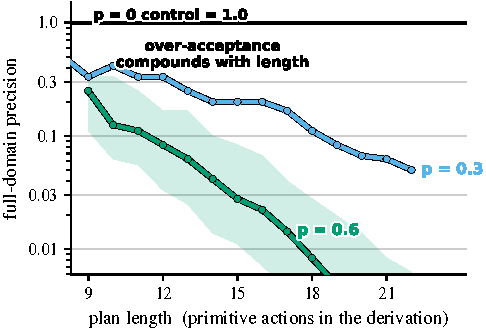
\includegraphics[width=\columnwidth]{figures/out/fig_compounding.pdf}
  \caption{Per-method over-acceptance compounds along the derivation, so
  full-domain precision decays geometrically with plan length---to $\sim\!1\%$
  valid on $22$-action UM-Translog plans---while the $p\!=\!0$ control stays
  exactly at $1.0$.}
  \label{fig:compound}
\end{figure}

% =====================================================================
%  In-text references (drop these sentences where each figure is discussed).
% =====================================================================
%
% The gap is not an artifact of single-action deletion but of a shared,
% re-used compound (Fig.~\ref{fig:leak}); across structurally-ambiguous
% families it is large and is exactly zero in the control (Fig.~\ref{fig:gap}).
% Crucially, it is nearly invisible to negatives drawn from the target plan
% --- zero under permutation, only a fraction under editing --- and surfaces in
% full only under gold-structural negatives (Fig.~\ref{fig:invisible}), which is
% why prior evaluations could not have seen it. A conformance-aware
% selector closes it at no cost to recall (Fig.~\ref{fig:gain}), and an
% independent temporal layer corroborates the same structure
% (Fig.~\ref{fig:timeline}). On the real IPC-2020 benchmark the effect is
% severe: the published SOTA repairs are a median $0.3\%$ valid at the target
% length (Fig.~\ref{fig:cliff}), because cost and precision are in tension and
% minimal cost sits at the precision floor (Fig.~\ref{fig:frontier}). The same
% over-acceptance is structurally a partial-order phenomenon: there,
% counter-examples recover gold ordering optimally (Fig.~\ref{fig:cegis}) and
% the local effect compounds with plan length (Fig.~\ref{fig:compound}).
